\def\CTeXPreproc{Created by ctex v0.2.12, don't edit!}\documentclass[aps,showpacs,superscriptaddress,twocolumn,prl]{revtex4}
\usepackage{mathrsfs}

\usepackage{amsmath}
\usepackage{amsfonts}
\usepackage{amssymb}
\usepackage{graphicx}
\usepackage{dcolumn}
\usepackage{bm}
\usepackage[colorlinks=true,dvipdfm]{hyperref}

\setcounter{MaxMatrixCols}{10}

\renewcommand{\textfraction}{0.15}
\renewcommand{\topfraction}{0.85}
\renewcommand{\bottomfraction}{0.65}
\renewcommand{\floatpagefraction}{0.60}
\begin{document}
\title{Experimental Implementation of a Quantum Random-Walk Search Algorithm Using Strongly Dipolar Coupled Spins}

\begin{abstract}
An important quantum search algorithm based on quantum random walk
performs an oracle search on a database of N items with
$\emph{O}(\sqrt{\emph{N}})$ calls, yielding a speed-up  similar to
the Grover's quantum search algorithm. We implemented the algorithm
on a three-qubit liquid-crystal nuclear magnetic resonance quantum
information processor in the case of finding 1-out-of-4, and
completed the diagonal elements' tomography of all the final density
matrices with comprehensible one dimensional NMR spectra. The
experimental results agree well with the theoretical predictions.
\end{abstract}

\pacs{03.65.Ud, 76.60.-k}\maketitle
\subsection*{I. Introduction}

Quantum computation has attracted much attention for the past decade
as quantum computers can efficiently solve significant series of
problems which are intractable for classical computers. The
computation tasks are rendered by algorithms. Since Shor's
remarkable factoring algorithm \cite{Shor}, many quantum algorithms
have been proposed. The algorithms presented early are mainly based
on quantum Fourier transform \cite{Shor} and Grover's search
algorithm \cite{Grover}. Later two alternative trends have entered
into the field, the adiabatic quantum algorithms \cite{Farhi} and
quantum random walk \cite{Aharonov,Farhi and Gutmann,Ambainis and
Back,Childs and Farhi,Childs and Cleve,Brun,Ambainis,Farhi and
Goldstone,Childs}. In this paper, we focus on the quantum-walk based search algorithm.

Since the classical random walk is a useful tool for developing classical algorithms, the quantum random
walk has been introduced as a potential method to formulate quantum algorithms. There are two distinct models, the continuous-time model and discrete-time model. The continuous-time model gives a unitary transformation directly in the space where the walk takes place. The discrete-time model requires an extra
coin register and defines a two-step procedure consisting of a quantum coin flip followed by a coin-controlled walk step. Investigations show that quantum random walks have notable different features to their classical counterparts \cite{Aharonov,Farhi and Gutmann}. These features may be used for designing quantum algorithms. Some relevant algorithms have been discovered within remarkable speedup over classical
computation \cite{Childs and Cleve,Shenvi}. The quantum search algorithm based on quantum random walk
proposed by Shenvi, Kempe, and Whaley (the SKW algorithm) \cite{Shenvi} is one of the novel algorithms, to perform an oracle search on a database of \emph{N} items with $\emph{O}(\sqrt{\emph{N}})$ calls, where \emph{N} is the size of the search space. Despite of a similar speed-up to the Grover's quantum search algorithm, the SKW algorithm is important as there are situations when the diffusion step of Grover's algorithm can not be implemented efficiently. Various optimizations and improvements of the SKW algorithm
have also been proposed in recent years \cite{Ambainis and Kempe,Tulsi,Reitzner,Chandrashekar,Potocek}, which can reduce the complexity and increase the search capability to a certain extent.

Some experiments about quantum random walk have been implemented in various physical systems for both continuous-time and discrete-time conditions \cite{Travaglione,Du,Ryan,Chandrashekar}, but as much as we know, hitherto no experiments about the algorithms based on quantum random walk have been reported. In this paper, we experimentally demonstrate the 1-out-of-4 case of the SKW algorithm \cite{Shenvi} and show its superiority over classical algorithms. The experiments are completed on a liquid-crystal nuclear magnetic resonance quantum information processor, with the strongly dipolar coupled Hamiltonian
\begin{eqnarray}\label{Hamiltonian}
\mathcal{H}=&&\sum\limits_j {\pi \nu _j } \sigma _z^j  + \sum\limits_{j < k} {\frac{\pi }{2}} J_{jk} \sigma _z^j \sigma _z^k \nonumber\\
&&+ \sum\limits_{j < k} {\frac{\pi }{2}} D_{jk} \left( {2\sigma _z^j \sigma _z^k  - \sigma _x^j \sigma _x^k  - \sigma _y^j \sigma _y^k } \right)
\end{eqnarray}
where $\nu_j$ is the resonance frequency of the \emph{j}th spin, $\emph{D}_{jk}$ and $\emph{J}_{jk}$ are the dipolar coupling strength and scalar coupling strength between spins \emph{j} and \emph{k}, respectively. The sums are restricted to the spins within one molecule. As not all the parts commute with each other, not all eigenstates are Zeeman product states but linear combinations of them. We still utilize the spins to store information but convert it to eigenbasis for more obvious and convenient tomography on NMR spectra. More details are described in Section III.

\subsection*{II. Algorithm}

First we give an overview of the original algorithm. Consider the unstructured search problem: given a function $\emph{f}\left(\emph{x}\right)$, $\emph{f}\left(\emph{x}\right)=1$ if $\emph{x}=\emph{a}$, otherwise $\emph{f}\left(\emph{x}\right)=0$. The goal is to find \emph{a}, where $0\leqslant \emph{a}\leqslant 2^n-1$. It is equivalent to search for a single marked node among the $\emph{N}=2^n$ nodes on the n-cube.

The discrete-time random walk can be described by the repeated application of a unitary evolution operator $U$. $U$ can be divided into two parts $U=SC$, where $S$ is a permutation matrix which performs a controlled shift based on the state of the coin space, and $C$ is a unitary matrix corresponding to "flipping" the quantum coin. To search the node, SKW introduce an oracle whose function is determined by the coin operator. The oracle will act by applying a marking coin $C_1$ to the marked node and the original coin $C_0$ to the unmarked nodes. This new coin operator is named $C'$. Then the perturbed unitary evolution operator $U'$ is given by $U'=SC'$ (see Fig.\ref{net}). After applying $U'$ for $t_{f}=\frac{\pi}{2}\sqrt{2^n}$ times, we will gain the marked state with probability $\frac{1}{2}-O(n)$ by measurement.

\begin{figure}[h] \centering
\includegraphics[width=\columnwidth]{net.eps}
\caption{\footnotesize{Quantum network for the algorithm in our 1-out-of-4 searching, with the target state being $\left\vert 11 \right\rangle_{23}$. The black dot represents 1-control gate while the white dot reversely. The purpose of $C'$ is to implement $C_1=R_x^1(\pi/2)$ (rotating qubit 1 around \emph{x} axis by angle $\pi/2$) when the "database" is $\left\vert 11 \right\rangle_{23}$ and $C_0=R_x^1(3\pi/2)$ otherwise. It is equivalent to be replaced by $R_1=R_x^1(3\pi/2)$ and $R_2=R_x^1(-\pi)$. The two controlled-not gates are inverting qubit 2 if qubit 1 is $\left\vert 1 \right\rangle_{1}$ and inverting qubit 3 if qubit 1 is $\left\vert 0 \right\rangle_{1}$,respectively. The measurement is all the populations', namely, diagonal elements' reconstruction. Similar circuits can be obtained straightforwardly for other target states. For instance if the goal is $\left\vert 10 \right\rangle_{23}$, we need only change the controlled condition of the three-body-interaction gate to state $\left\vert 10 \right\rangle_{23}$.}}\label{net}
\end{figure}

When $n=2$, three qubits are needed to demonstrate the algorithm. One qubit is used as the "coin" (referred as the "coin qubit", labeled by qubit 1), while the other two are used as the database (referred as the "database qubits", labeled by qubit 2 and 3). The target state is $\left\vert \tau\sigma \right\rangle_{23} = \left\vert \tau \right\rangle_{2}\otimes\left\vert \sigma \right\rangle_{3} \left(\tau,\sigma=0,1 \right)$ out of the four computational basis ${\left\vert 00 \right\rangle_{23},\left\vert 01 \right\rangle_{23},\left\vert 10 \right\rangle_{23},\left\vert 11 \right\rangle_{23}}$. The 1-out-of-4 algorithm is implemented as the network shown in Fig.\ref{net}. Without of loss generality, suppose the initial state is $\left\vert 111 \right\rangle$.

(i) Prepare the state
\begin{equation} \label{initial}
\left\vert \psi_{i} \right\rangle=\frac{\left\vert 0 \right\rangle_1-\left\vert 1 \right\rangle_1}{\sqrt{2}}\otimes\frac{\left\vert 0 \right\rangle_2-\left\vert 1 \right\rangle_2}{\sqrt{2}}\otimes\frac{\left\vert 0 \right\rangle_3-\left\vert 1 \right\rangle_3}{\sqrt{2}},
\end{equation}
which is exactly an equal superposition over all the computational basis. It is simple to do this by applying a Hadamard operation to every qubit.

(ii) On each step, the "coin qubit" undergose a unitary operation depending on the state of "database qubits", namely, $C_1=R_x^1(\pi/2)=e^{-i\pi\sigma_x/4}$ if the "database qubits" are on the target state $\left\vert \tau\sigma \right\rangle_{23}$, and $C_0=R_x^1(3\pi/2)=e^{-i3\pi\sigma_x/4}$ otherwise (In Fig.\ref{net}, this controlled operation is simplified through $R_1=R_x^1(3\pi/2)=e^{-i3\pi\sigma_x/4}$ and $R_2=R_x^1(-\pi)=e^{i\pi\sigma_x/2}$ equivalently). Therefore the whole "coin" operation is
\begin{equation} \label{C'}
C'=C_0\otimes E_{23}+(C_1-C_0)\otimes\left\vert \tau\sigma \right\rangle_{2323}\left\langle \tau\sigma \right\vert
\end{equation}
where $E_{23}$ is the identity operator on the "database qubits". Then the "database qubits" undergo the shift operation $S$ conditioned on the state of "coin qubit":
\begin{eqnarray}\label{S}
&&\left\vert 0 \right\rangle_{1}\left\vert 00 \right\rangle_{23}\Longleftrightarrow\left\vert 0 \right\rangle_{1}\left\vert 01 \right\rangle_{23} \nonumber\\
&&\left\vert 0 \right\rangle_{1}\left\vert 10 \right\rangle_{23}\Longleftrightarrow\left\vert 0 \right\rangle_{1}\left\vert 11 \right\rangle_{23} \nonumber\\
&&\left\vert 1 \right\rangle_{1}\left\vert 00 \right\rangle_{23}\Longleftrightarrow\left\vert 1 \right\rangle_{1}\left\vert 01 \right\rangle_{23} \nonumber\\
&&\left\vert 1 \right\rangle_{1}\left\vert 01 \right\rangle_{23}\Longleftrightarrow\left\vert 1 \right\rangle_{1}\left\vert 11 \right\rangle_{23}
\end{eqnarray}

(iii) After repeating step (ii) twice, it reaches the final state
\begin{equation} \label{final}
\left\vert \psi_{f} \right\rangle=\left( SC' \right)^2 \left\vert \psi_{i} \right\rangle
\end{equation}
For example, in the case of finding $\left\vert 111 \right\rangle_{23}$, $\left\vert \psi_{f} \right\rangle$ is specialized as
\begin{equation} \label{final}
\left\vert \psi_{f} \right\rangle=\frac{\sqrt{2}}{4} \left\vert 001 \right\rangle+\frac{\sqrt{2}}{4} \left\vert 101 \right\rangle+\frac{\sqrt{2}}{4} \left\vert 010 \right\rangle+\frac{\sqrt{2}}{4} \left\vert 110 \right\rangle+\frac{\sqrt{2}}{2} \left\vert 011 \right\rangle
\end{equation}
Through this expression we can obtain the theoretic probabilities of ${\left\vert 00 \right\rangle_{23},\left\vert 01 \right\rangle_{23},\left\vert 10 \right\rangle_{23},\left\vert 11 \right\rangle_{23}}$ are 0, 0.25, 0.25, 0.5 correspondingly after tracing qubit 1 out.

For other target states, similar circuits can be given easily with the controlled condition changed. The theoretic results have an analogy with the above.

\subsection*{II. Implementation}

\subsubsection*{\textbf{A. System}}

To implement the algorithm we used the three ${}^1 H$ spins in a
sample of 1-Bromo-2,3-Dichlorobenzene oriented in liquid-crystal
solvent ZLI-1132. All experiments were conducted on a Bruker Avance
500 MHz spectrometer at room temperature. The molecular structure is
shown in Fig.\ref{energy_level}(a). The internal Hamiltonian of this
system can be described as
\begin{eqnarray}\label{Hamiltonian}
\mathcal{H}=&&\sum\limits_{j=1}^3 {\pi \nu _j } \sigma _z^j  + \sum\limits_{j,k,j < k\leqslant 3} {\frac{\pi }{2}} J_{jk} \sigma _z^j \sigma _z^k \nonumber\\
&&+ \sum\limits_{j,k,j < k\leqslant 3} {\frac{\pi }{2}} D_{jk} \left( {2\sigma _z^j \sigma _z^k  - \sigma _x^j \sigma _x^k  - \sigma _y^j \sigma _y^k } \right)
\end{eqnarray}
The spectrum of the thermal equilibrium state
$\rho_{th}=\sum\limits_{i=1}^3 \sigma_z^i$ applying a $\pi/2$ hard
pulse is shown in Fig.\ref{energy_level}(b). With some initially
guessed parameters (chemical shifts, scalar coupling constants and
dipolar coupling constants), we iteratively fit the calculated and
observed spectra through the parameters' perturbation. All the
calculated values are listed in Table. \ref{para} (a).

\begin{table}[htb] \centering
\includegraphics[width=0.9\columnwidth]{para.eps}
\caption{\footnotesize{(Color online)(a) The Hamiltonian parameters
of 1-Bromo-2,3-Dichlorobenzene. The diagonal elements are chemical
shifts of the three protons, the off-diagonal elements above (red)
are dipolar coupling strengths while below (sky-blue) represent
scalar coupling strengths. (b) The read-out pulses and corresponding
values of $P(i)-P(j)$. The results are showed on transition No.9, 8
and 7. Combined with the normalized condition $\sum_{i=1}^8=1$, all
the diagonal elements can be solved.}}\label{para}
\end{table}

With the system Hamiltonian confirmed, we consider the procedure of diagonalizing the Hamiltonian. It is not difficult to find a feasible unitary matrix $U$ to equalize
\begin{equation} \label{diag}
H_L = UH_SU^{\dag}
\end{equation}
where $H_S$ is the system Hamiltonian and $H_L$ is one diagonal
Hamiltonian. Specially, for the system Hamiltonian mentioned above,
the transformation $U$ we have selected is

\begin{eqnarray}\label{Transformation}
\left( {\begin{array}{*{20}c}
   {1} & {0} & {0} & {0} & {0} & {0} & {0} & {0}  \\
   {0} & {0.8009} & {0.5166} & {0} & {-0.3028} & {0} & {0} & {0}  \\
   {0} & {0.3745} & {-0.8267} & {0} & {-0.4199} & {0} & {0} & {0}  \\
   {0} & {0} & {0} & {0.8197} & {0} & {0.1260} & {0.5588} & {0}  \\
   {0} & {-0.4673} & {0.2229} & {0} & {-0.8556} & {0} & {0} & {0}  \\
   {0} & {0} & {0} & {0.4584} & {0} & {-0.7294} & {-0.5078} & {0}  \\
   {0} & {0} & {0} & {0.3436} & {0} & {0.6724} & {-0.6556} & {0}  \\
   {0} & {0} & {0} & {0} & {0} & {0} & {0} & {1}  \\
\end{array}} \right)
\end{eqnarray}

which is one of the $8!=40320$ feasible unitary matrices that can
diagonalize the Hamiltonian. Through this labeling scheme all the
transitions are between two eigenstates in $\left\vert 000
\right\rangle_L$ ~ $\left\vert 111 \right\rangle_L$ with $\left\vert
000 \right\rangle_L=\left\vert 000 \right\rangle_S,\left\vert 111
\right\rangle_L=\left\vert 111 \right\rangle_S$. The nine observable
transitions in the thermal equilibrium spectrum are marked in the
transition diagram (Fig.\ref{energy_level}(c)).

\begin{figure}[h] \centering
\includegraphics[width=\columnwidth]{energy_level.eps}
\caption{\footnotesize{(Color online)(a) The molecular structure of
1-Bromo-2,3-Dichlorobenzene with the three protons forming 3-qubit
system. (b) The spectrum of the thermal equilibrium state
$\rho_{th}=\sum_{i=1}^3 \sigma_z^i$ applying a $\pi/2$ hard pulse.
All the transitions are labeled according to the descending orders
of the frequencies. (c) The correspondingly transition diagram in
the $H_L$ picture. The red (No.1 and No.9), green (No.2 and No.8),
yellow (No.3 and No.7) lines express the transitions of qubit 1, 2
and 3 in the $H_L$ picture, respectively.}}\label{energy_level}
\end{figure}

Without loss of generality, we focused on the right three
transitions No.7, 8 and 9, which cover all the three qubits'
single-quantum transitions. Considering a simple case that $\rho_S$
is a pure state $(\left\vert 000 \right\rangle\left\langle 000
\right\vert)_S$. In the Ising model, if the transition of qubit 1 is
excited (a selective pulse $R_1^y(\pi/2)$ is enough), a single peak
can be obtained in the spectrum. This is a universal way to test the
created pseudo pure state on liquid NMR. However, in the current
Heisenberg model, since the Hamiltonian's noncommunity, a single
qubit rotation will not lead to a single peak but combination of
some relative peaks (see the left column of Fig.aaaaaaaaaaaaaa). The
complicated spectrum is obviously not proper to read out the
information of density matrix. A straight idea to solve the problem
is to utilize the $H_L$ picture where the Hamiltonian is an Ising
type. From Eq.\ref{diag} we can clearly see that add the
transformation matrix $U$ before the read-out pulse is all right.
The right column of Fig. aaaaaaaaaaa shows the spectra of
$(\left\vert 000 \right\rangle\left\langle 000 \right\vert)_S$ with
three read-out pulses
$UR_1^y(\pi/2),UR_2^y(\pi/2)R_3^y(\pi),UR_3^y(\pi/2)$. The second
pulse needs a $R_3^y(\pi)$ rotation as transition No.8 represents
$\left\vert 001 \right\rangle_L\rightarrow \left\vert 011
\right\rangle_L$, not $\left\vert 000 \right\rangle_L\rightarrow
\left\vert 010 \right\rangle_L$. The simulating spectra accord well
with the expected results, similarly to the Ising type.

For reading-out the diagonal elements of a general density matrix
$\rho_S$, the method above is still effective. Suppose the
populations of $(\left\vert 000 \right\rangle\left\langle 000
\right\vert)_S$~$(\left\vert 111 \right\rangle\left\langle 111
\right\vert)_S$ are $P(1)$~$P(8)$, $UR_1^y(\pi/2)$ would excite the
transitions $\left\vert 000 \right\rangle_L\rightarrow \left\vert
100 \right\rangle_L$ and $\left\vert 100 \right\rangle_L\rightarrow
\left\vert 000 \right\rangle_L$, displayed on transition No.9.
Compared with the integration of the pure-state case, we can obtain
the value of $P(1)-P(5)$. Table. \ref{para} (b) shows all the
available values of $P(i)-P(j)$ through different read-out pulses.
Combined with the normalization condition $\sum_{i=1}^8P(i)=1$, all
the eight population values can be calculated. Now we have
accomplished the diagonal elements' tomography.

\subsubsection*{\textbf{B. Experiment}}

The experiment was divided into three steps: the psesudo-pure state
preparation, quantum random walk searching process, and populations'
measurement. Starting from the thermal equilibrium state, firstly we
need to create the PPS $\rho_{000}=\frac{1-\epsilon
}{8}\mathbf{1}+\epsilon \left\vert 000 \right\rangle \left\langle
000\right\vert$, where $\epsilon$ represents the polarization of the
system and $\mathbf{1}$ is the identity matrix. We used strongly
modulating pulses based on GRadient Ascent Pulse Engineering (GRAPE)
algorithm \cite{GRAPE} and gradient pulses to realize the PPS
preparation, with the numerical simulated fidelity 97.7%.

\begin{figure}[h] \centering
\includegraphics[width=\columnwidth]{aaa.eps}
\caption{\footnotesize{(Color online)(a) The molecular structure of
1-Bromo-2,3-Dichlorobenzene with the three protons forming 3-qubit
system. (b) The spectrum of the thermal equilibrium state
$\rho_{th}=\sum_{i=1}^3 \sigma_z^i$ applying a $\pi/2$ hard pulse.
All the transitions are labeled according to the descending orders
of the frequencies. (c) The correspondingly transition diagram in
the $H_L$ picture. The red (No.1 and No.9), green (No.2 and No.8),
yellow (No.3 and No.7) lines express the transitions of qubit 1, 2
and 3 in the $H_L$ picture, respectively.}}\label{energy_level}
\end{figure}


\begin{thebibliography}{99}
\bibitem{Shor} P. W. Shor, SIAM J. Comput. \textbf{26}, 1484 (1997).
\bibitem{Grover} L. Grover,Phys. Rev. Lett. \textbf{79}, 325 (1997).
\bibitem{Farhi} Farhi E, Goldstone J, Gutmann S, Lapan J, Lundgren A, and Preda D, Science \textbf{292},412 (2001).
\bibitem{Aharonov} Y. Aharonov, L. Davidovich, and N. Zagury, Phys. Rev. A \textbf{48}, 1687 (1993).
\bibitem{Farhi and Gutmann} E. Farhi and S. Gutmann, Phys. Rev. A \textbf{58}, 915 (1998).
\bibitem{Ambainis and Back} A. Ambainis, E. Back, A. Nayak, A. Vishwanath, and J. Watrous, in \emph{Proceedings of the 30th
annual ACM Symposium on Theory of Computing} (Association for
Computing Machinery, New York, 2001), pp. 60-69.
\bibitem{Childs and Farhi} A. Childs, E. Farhi, and S. Gutmann, Quantum Inform. Process.
\textbf{1}, 35 (2002).
\bibitem{Childs and Cleve} A. Childs, R. Cleve, E. Deotto, E. Farhi, S. Gutmann, and D.
Spielman, Proc. 35th ACM Symposium on The- ory of Computing (STOC
2003), pp. 59-68.
\bibitem{Brun} T. A. Brun, H. A. Carteret and A. Ambainis, Phys. Rev. Lett. \textbf{91}, 130602 (2003).
\bibitem{Ambainis} A. Ambainis, SIAM J. Comput. \textbf{37}, 210 (2007).
\bibitem{Farhi and Goldstone} E. Farhi, J. Goldstone, and S. Gutmann, Theory Comput.
\textbf{4}, 169 (2008).
\bibitem{Childs} A. Childs, Phys. Rev. Lett. \textbf{102}, 180501 (2008).
\bibitem{Shenvi} N. Shenvi, J. Kempe and K. B. Whaley, Phys. Rev. A \textbf{67},
052307 (2003).
\bibitem{Ambainis and Kempe} A. Ambainis, J. Kempe, and A. Rivosh, \emph{Proceedings of the
16th ACM-SIAM SODA} (Society for Industrial and Applied
Mathematics, Philadelphia, 2005), pp. 1099 �C~1108.
\bibitem{Tulsi} A. Tulsi, Phys. Rev. A \textbf{78}, 012310 (2008).
\bibitem{Reitzner} D. Reitzner, M. Hillery, E. Feldman, and V. Bu$\check{z}$ek, Phys. Rev. A \textbf{79}, 012323 (2009).
\bibitem{Chandrashekar} C. M. Chandrashekar, R. Srikanth, and R. Laflamme, Phys.
Rev. A \textbf{77}, 032326 (2008).
\bibitem{Potocek} V. Poto$\check{c}$ek, A. G$\acute{a}$bris, T. Kiss and I. Jex, Phys.
Rev. A \textbf{79}, 012325 (2009).
\bibitem{Travaglione} B. C. Travaglione and G. J. Milburn, Phys. Rev. A \textbf{65},
032310 (2002).
\bibitem{Du} J. Du et al., Phys. Rev. A \textbf{67}, 042316 (2003).
\bibitem{Ryan} C. A. Ryan, M. Laforest, J. C. Boileau, and R. Laflamme,
Phys. Rev. A \textbf{72}, 062317 (2005).
\bibitem{Chandrashekar} C. M. Chandrashekar, Phys. Rev. A \textbf{74}, 032307 (2006).
\bibitem{GRAPE} J. Baugh et al., Phys. in Can. \textbf{63}, No.4
(2007), 'Special issue on quntum information and quantum computing';
N. Khaneja et al., J. Magn. Reson. \textbf{172}, 296 (2005); C. A.
Ryan et al., Phys. Rev. A \textbf{78}, 012328 (2008).
\end{thebibliography}

\end{document}
